% Exercise ID: MAT_P4FUNCOE_0PX_IGX_001
% Created: 2025-11-26
% Difficulty: 1/5

\exercicio{
Observe o retângulo representado no plano cartesiano abaixo, limitado pelos intervalos $[1,4]$ no eixo dos $x$ e $[2,5]$ no eixo dos $y$. Escreva o produto cartesiano de intervalos que representa este conjunto de pontos.

\begin{center}
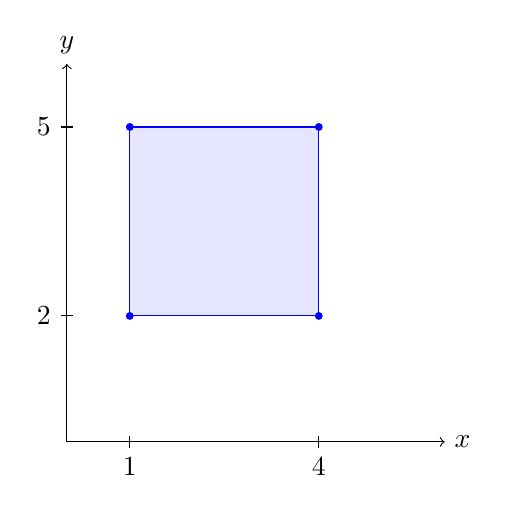
\begin{tikzpicture}[scale=0.8]
    % Eixos
    \draw[->] (0,0) -- (6,0) node[right] {$x$};
    \draw[->] (0,0) -- (0,6) node[above] {$y$};
    % Retângulo preenchido
    \filldraw[fill=blue!10,draw=blue] (1,2) rectangle (4,5);
    % Marcas nos eixos
    \foreach \x in {1,4}
        \draw (\x,0.1) -- (\x,-0.1) node[below] {\x};
    \foreach \y in {2,5}
        \draw (0.1,\y) -- (-0.1,\y) node[left] {\y};
    % Pontos dos vértices
    \foreach \x/\y in {1/2, 1/5, 4/2, 4/5}
        \filldraw[blue] (\x,\y) circle (1.5pt);
\end{tikzpicture}
\end{center}
}
